% =================================================================
% Trabajo Final Integrador — Tópicos en Aprendizaje Automático (UNAJ)
% Análisis crítico y réplica parcial de "Patches Are All You Need?"
% Estética UNAJ (la de la presentación de Metodología I). Compilar con
% pdflatex (dos pasadas). Números: resultados.tex (src/figuras.py).
% =================================================================
\documentclass[aspectratio=169,xcolor=table]{beamer}

\usepackage{iftex}
\ifPDFTeX
  \usepackage[utf8]{inputenc}
  \usepackage[T1]{fontenc}
  \usepackage{lmodern}
\else
  \usepackage{fontspec}
\fi
\usepackage[spanish,es-noshorthands,es-nodecimaldot,es-tabla]{babel}
\usepackage{booktabs}
\usepackage{array}
\usepackage{tabularx}
\usepackage{amsmath}
\usepackage{tikz}
\usetikzlibrary{arrows.meta,positioning,shapes.geometric,fit,calc}
\graphicspath{{figuras/}}
% Generado por src/figuras.py a partir de results/*.json — no editar a mano
\providecommand{\accCMnueve}{82,7}
\providecommand{\paramsCMnueve}{223\,370}
\providecommand{\tputCMnueve}{422}
\providecommand{\minCMnueve}{110}
\providecommand{\valCMnueve}{83,1}
\providecommand{\entrCMnueve}{84,6}
\providecommand{\accCMtres}{84,6}
\providecommand{\paramsCMtres}{149\,642}
\providecommand{\tputCMtres}{531}
\providecommand{\minCMtres}{72}
\providecommand{\valCMtres}{85,4}
\providecommand{\entrCMtres}{86,2}
\providecommand{\accCMpcuatro}{78,7}
\providecommand{\paramsCMpcuatro}{227\,978}
\providecommand{\tputCMpcuatro}{1551}
\providecommand{\minCMpcuatro}{35}
\providecommand{\valCMpcuatro}{78,7}
\providecommand{\entrCMpcuatro}{78,8}
\providecommand{\accResNet}{83,0}
\providecommand{\paramsResNet}{308\,650}
\providecommand{\tputResNet}{1572}
\providecommand{\minResNet}{32}
\providecommand{\valResNet}{83,1}
\providecommand{\entrResNet}{83,7}
\providecommand{\epocasCNN}{10}
\providecommand{\accLineal}{40,7}
\providecommand{\lamCV}{10000}
\providecommand{\minLineal}{148}
\providecommand{\accPerceptron}{40,3}
\providecommand{\minPerceptron}{1}
\providecommand{\accMLP}{57,4}
\providecommand{\paramsMLP}{3\,676\,682}
\providecommand{\tputMLP}{14147}
\providecommand{\minMLP}{4}
\providecommand{\accELM}{47,3}
\providecommand{\LELM}{3000}
\providecommand{\paramsELM}{9\,249\,000}
\providecommand{\minELM}{3}
\providecommand{\accMLELM}{40,4}
\providecommand{\minMLELM}{9}
\providecommand{\ratioTput}{3,7}
\providecommand{\difCMResNet}{-0,3}
\providecommand{\difKernel}{-2,0}
\providecommand{\difKernelAbs}{2,0}
\providecommand{\difPatch}{4,0}
\providecommand{\accColab}{94,5}
\providecommand{\segColab}{56}
\providecommand{\epColab}{100}
\providecommand{\minColab}{93}
\providecommand{\minEpCPU}{11}
\providecommand{\colabNota}{al cabo de las 100 épocas}
\providecommand{\accKaggle}{95,48}
\providecommand{\segKaggle}{25}
\providecommand{\epKaggle}{200}
\providecommand{\minKaggle}{85}


% -----------------------------------------------------------------
% Estética UNAJ
% -----------------------------------------------------------------
\definecolor{unajazul}{HTML}{003366}
\definecolor{unajgris}{HTML}{E6E6E6}
\definecolor{unajnaranja}{HTML}{D9822B}
\definecolor{unajrojo}{HTML}{C0392B}

\usetheme{default}
\setbeamertemplate{navigation symbols}{}
\setbeamercolor{structure}{fg=unajazul}
\setbeamercolor{title}{fg=white,bg=unajazul}
\setbeamercolor{subtitle}{fg=white}
\setbeamercolor{frametitle}{fg=unajazul,bg=unajgris}
\setbeamercolor{block title}{fg=white,bg=unajazul}
\setbeamercolor{block body}{fg=black,bg=unajgris}
\setbeamercolor{block title alerted}{fg=white,bg=unajazul!75!black}
\setbeamercolor{block body alerted}{fg=black,bg=unajgris}
\setbeamercolor{block title example}{fg=white,bg=unajnaranja!85!black}
\setbeamercolor{block body example}{fg=black,bg=unajgris}
\setbeamercolor{author in head/foot}{fg=unajazul}
\setbeamercolor{title in head/foot}{fg=black}
\setbeamercolor{date in head/foot}{fg=unajazul!75}
\setbeamerfont{footline}{size=\tiny}
\setbeamertemplate{itemize items}[triangle]
\setbeamertemplate{enumerate items}[default]

\setbeamertemplate{footline}{%
  \leavevmode%
  \hbox{%
    \begin{beamercolorbox}[wd=.333333\paperwidth,ht=2.6ex,dp=1.6ex,center]{author in head/foot}%
      \usebeamerfont{footline}\insertshortauthor
    \end{beamercolorbox}%
    \begin{beamercolorbox}[wd=.333333\paperwidth,ht=2.6ex,dp=1.6ex,center]{title in head/foot}%
      \usebeamerfont{footline}\insertshorttitle
    \end{beamercolorbox}%
    \begin{beamercolorbox}[wd=.333333\paperwidth,ht=2.6ex,dp=1.6ex,right]{date in head/foot}%
      \usebeamerfont{footline}\insertshortdate\hspace*{2em}%
      \insertframenumber{} / \inserttotalframenumber\hspace*{2ex}
    \end{beamercolorbox}}%
  \vskip0pt%
}

\newcommand{\fuente}[1]{\vfill{\fontsize{5.5}{6.5}\selectfont\color{gray}#1\par}}
\newcommand{\bignum}[2]{%
  \begin{minipage}[t]{\linewidth}\centering
    {\fontsize{26}{28}\selectfont\bfseries\color{unajazul}#1}\\[0.2em]
    {\scriptsize #2}
  \end{minipage}}
\newcommand{\clave}[1]{\vfill\begin{alertblock}{Clave}\footnotesize #1\end{alertblock}}
\newcommand{\figslide}[3]{%
  \begin{frame}{#1}
    \centering
    \includegraphics[width=0.95\textwidth,height=0.72\textheight,keepaspectratio]{#2}\\[-0.1em]
    {\scriptsize #3}
  \end{frame}}

% -----------------------------------------------------------------
\newcommand{\fechaexpo}{Diciembre de 2026}
\title[TF: ¿Bastan los parches? (ConvMixer)]{¿Bastan los parches?}
\subtitle{Análisis crítico y réplica parcial de \emph{Patches Are All You Need?}\\
  (Trockman y Kolter, TMLR 2023)}
\author[Marcos Kantor]{Marcos David Kantor\\[2pt]
  {\small Docentes: Dr.\ Ing.\ Martín Morales y Dr.\ Ing.\ Marcelo Cappelletti}}
\institute[UNAJ]{Universidad Nacional Arturo Jauretche --- Doctorado en Ciencia y Tecnología\\
  Curso de posgrado: Tópicos en Aprendizaje Automático --- Trabajo Final Integrador}
\date[\fechaexpo]{\fechaexpo}
\titlegraphic{
\includegraphics[height=1.45cm]{logo_unaj.png}}
\hypersetup{pdftitle={¿Bastan los parches? Análisis crítico del ConvMixer}, pdfauthor={Marcos David Kantor}}

\begin{document}

% =================================================================
\begin{frame}[plain]
  \vspace*{-2pt}
  \titlepage
\end{frame}

% =================================================================
\begin{frame}{Contenido de la exposición}
  \begin{columns}[T]
    \begin{column}{.52\textwidth}
      \begin{enumerate}
        \item \textbf{El artículo} y por qué cumple la consigna.
        \item \textbf{Introducción}: el problema y la motivación.
        \item \textbf{Explicación teórica} del ConvMixer.
        \item \textbf{Metodología} de los autores.
        \item \textbf{Resultados} y \textbf{conclusiones} del artículo.
        \item \textbf{Réplica parcial} en CIFAR-10, comparada con modelos de las cinco unidades.
        \item \textbf{Reflexión crítica}.
      \end{enumerate}
    \end{column}
    \begin{column}{.44\textwidth}
      \begin{block}{En una frase}
        \small Una red convolucional de seis líneas, que recibe la imagen en \emph{parches} como el ViT, compite
        con los transformers: parte del mérito estaría en los parches y no en la atención.
      \end{block}
      \vspace{4pt}
      \bignum{\accCMnueve\,\%}{ConvMixer-128/8 en CIFAR-10, réplica en CPU, \epocasCNN{} épocas\\(paper: 95,0\,\% con 256/8 y 200 épocas en GPU)}
    \end{column}
  \end{columns}
  \fuente{Exposición de 20 minutos + 10 de debate.}
\end{frame}

% =================================================================
\section{El artículo}
\begin{frame}{El artículo seleccionado}
  \begin{columns}[T]
    \begin{column}{.56\textwidth}
      \textbf{Trockman, A. y Kolter, J. Z.} (Carnegie Mellon / Bosch Center for AI)\\
      \emph{Patches Are All You Need?}\\
      Transactions on Machine Learning Research, 2023 --- arXiv:2201.09792 (2022)\\
      Código: \texttt{github.com/locuslab/convmixer}
      \vspace{6pt}
      \begin{block}{Cumple la consigna}
        \small
        \begin{itemize}
          \item Reciente (2022--2023) y con un problema relevante: clasificación de imágenes.
          \item Propone un modelo y lo compara con ResNet, ViT, DeiT, MLP-Mixer, ResMLP y Swin.
          \item Resultados en ImageNet-1k y CIFAR-10, este último \textbf{público y replicable}.
        \end{itemize}
      \end{block}
    \end{column}
    \begin{column}{.40\textwidth}
      \begin{block}{Ubicación en el programa}
        \small
        \textbf{U4 (CNN)}: convoluciones 2D, SGD, arquitecturas y modelos.\\[3pt]
        La réplica agrega un modelo de cada unidad: \textbf{U1} validación cruzada, \textbf{U2} seudoinversa
        y perceptrón, \textbf{U3} MLP, \textbf{U5} ELM y ML-ELM.
      \end{block}
      \vspace{3pt}
      {\footnotesize Es bibliografía de la materia \emph{Sistemas de Inteligencia Artificial} (ITBA) que cursé
      en paralelo.}
    \end{column}
  \end{columns}
\end{frame}

% =================================================================
\section{Introducción}
\begin{frame}{El problema: el ViT cambió dos cosas a la vez}
  \begin{columns}[T]
    \begin{column}{.5\textwidth}
      \begin{block}{CNN clásica (ResNet; He et al., 2016)}
        \small Ve píxeles. Es \textbf{piramidal}: la resolución baja y los canales suben capa a capa.
        Su sesgo inductivo es la localidad y los pesos compartidos.
      \end{block}
      \vspace{4pt}
      \begin{block}{Vision Transformer (2021)}
        \small (Dosovitskiy et al., 2021). Corta la imagen en \textbf{parches} de $16\times16$ (la atención cuesta
        $O(n^2)$). Es \textbf{isotrópico}: igual resolución y ancho en todas las capas.
      \end{block}
    \end{column}
    \begin{column}{.46\textwidth}
      \begin{alertblock}{Pregunta del artículo}
        \small ¿El ViT rinde por el \emph{transformer} o, al menos en parte, porque usa \textbf{parches} como
        representación?
      \end{alertblock}
      \vspace{4pt}
      {\footnotesize\textbf{Por qué importa}: es una pregunta sobre el \emph{sesgo inductivo}. Si los parches
      explican la mejora, se conserva la eficiencia de datos de la convolución sin el costo de la atención: clave
      con pocos datos, como en imágenes médicas.}\\[4pt]
      {\footnotesize\textbf{Motivación}: el modelo \emph{más simple} que conserve lo que comparten ViT y
      MLP-Mixer, con la atención reemplazada por la operación menos expresiva: la convolución.}
    \end{column}
  \end{columns}
\end{frame}

% =================================================================
\section{Modelo}
\begin{frame}{El ConvMixer: parches + mezcla espacial + mezcla de canales}
  \centering
  \begin{tikzpicture}[node distance=4mm, every node/.style={font=\scriptsize},
      caja/.style={draw=unajazul, fill=unajgris, rounded corners=2pt, minimum height=7mm, align=center, inner sep=3pt},
      flecha/.style={-{Stealth[length=2mm]}, thick, unajazul}]
    \node[caja] (img) {Imagen\\$3\times n\times n$};
    \node[caja, right=of img] (pe) {\textbf{Parches}\\Conv $p\times p$, paso $p$\\GELU, BN};
    \node[caja, right=8mm of pe, minimum width=26mm] (dw) {\textbf{Depthwise} $k\times k$\\(un filtro por canal)\\GELU, BN};
    \node[caja, right=8mm of dw] (pw) {\textbf{Pointwise} $1\times1$\\(mezcla canales)\\GELU, BN};
    \node[caja, right=of pw] (gap) {Pooling\\global};
    \node[caja, right=of gap] (fc) {Lineal\\softmax};
    \draw[flecha] (img) -- (pe);
    \draw[flecha] (pe) -- (dw);
    \draw[flecha] (dw) -- (pw);
    \draw[flecha] (pw) -- (gap);
    \draw[flecha] (gap) -- (fc);
    \draw[flecha, unajnaranja] ($(pe.east)+(3mm,0)$) |- ++(0,10mm) -| ($(dw.east)+(3mm,0)$) node[pos=0.25, above, text=black] {residual};
    \node[draw=unajazul, dashed, rounded corners, fit=(dw)(pw), inner sep=5mm, label={[text=unajazul]below:{$\times\,d$ bloques idénticos, sin submuestreo (isotrópico)}}] {};
  \end{tikzpicture}
  \vspace{4pt}
  \begin{columns}[T]
    \begin{column}{.5\textwidth}
      \small
      $z_0=\mathrm{BN}(\sigma\{\mathrm{Conv}_{c\to h}(X,\ \text{stride}{=}p,\ \text{kernel}{=}p)\})$\\[2pt]
      $z'_l=\mathrm{BN}(\sigma\{\mathrm{ConvDepthwise}(z_{l-1})\})+z_{l-1}$\\[2pt]
      $z_{l+1}=\mathrm{BN}(\sigma\{\mathrm{ConvPointwise}(z'_l)\})$
    \end{column}
    \begin{column}{.46\textwidth}
      \small
      \textbf{ConvMixer-$h$/$d$}: ancho $h$, profundidad $d$, parche $p$, núcleo $k$.\\
      $\#\theta=h[d(k^2+h+6)+c\,p^2+n+3]+n$ (ec.~4)\\
      Núcleos \textbf{grandes} ($k=7$--$9$) para mezclar posiciones lejanas, como la atención.
    \end{column}
  \end{columns}
  \fuente{\textit{Nota.} Elaboración propia a partir de Trockman y Kolter (2023, Fig.~2 y ecs.~1--4). Aprendizaje supervisado; entropía cruzada; AdamW.}
\end{frame}

\begin{frame}{Cómo encaja con la Unidad 4, y qué no vimos en el curso}
  \begin{columns}[T]
    \begin{column}{.48\textwidth}
      \begin{block}{Lo que es de la U4}
        \small
        \begin{itemize}
          \item Conv 2D discreta: el \emph{embebido de parches} es una conv con paso $=$ núcleo.
          \item \emph{Depthwise} + \emph{pointwise} = conv separable (MobileNet).
          \item SGD (AdamW), BatchNorm y conexión residual.
          \item Campo receptivo: $p\,[1+d(k-1)]$ píxeles.
        \end{itemize}
      \end{block}
    \end{column}
    \begin{column}{.48\textwidth}
      \begin{exampleblock}{Comparados que no se ven en el curso}
        \small
        \textbf{ViT/DeiT} (Touvron et al., 2021): \emph{transformer} sobre parches; cada parche pondera a todos los demás
        ($\mathrm{softmax}(QK^\top/\sqrt d)V$).\\[2pt]
        \textbf{MLP-Mixer} (Tolstikhin et al., 2021) \textbf{/ResMLP}: una MLP mezcla parches y otra mezcla canales.\\[2pt]
        \textbf{Swin} (Liu et al., 2021): transformer jerárquico con ventanas locales.
      \end{exampleblock}
    \end{column}
  \end{columns}
  \clave{El ConvMixer es un MLP-Mixer con convoluciones en lugar de MLP. Si rinde parecido, lo que importa es lo
  que comparten: parches y diseño isotrópico.}
\end{frame}

% =================================================================
\section{Metodología}
\begin{frame}{Metodología de los autores}
  \begin{columns}[T]
    \begin{column}{.5\textwidth}
      \small
      \textbf{Datos}: ImageNet-1k (1,28\,M imágenes, 1\,000 clases, $224^2$) y CIFAR-10 (50\,k + 10\,k,
      $32^2$, 10 clases). Sin pre-entrenamiento.\\[3pt]
      \textbf{Preprocesamiento}: normalización y aumentación intensa con \texttt{timm}: RandAugment, mixup,
      CutMix, \emph{random erasing}, escalado aleatorio.\\[3pt]
      \textbf{Características}: no hay selección explícita; los parches \emph{aprenden} los filtros.\\[3pt]
      \textbf{Partición}: la estándar; informan sobre la validación de ImageNet y el test de CIFAR-10.
    \end{column}
    \begin{column}{.46\textwidth}
      \small
      \textbf{Entrenamiento}: AdamW, tasa de aprendizaje triangular, recorte de la norma del gradiente; 90--300
      épocas (unos 9 días en 10 GPU) y 200 en CIFAR-10.\\[3pt]
      \textbf{Hiperparámetros}: ``\emph{absolutamente ninguna}'' búsqueda en ImageNet; en CIFAR-10, barrido manual
      de $h, d, p, k$ y \emph{weight decay}.\\[3pt]
      \textbf{Métricas}: exactitud top-1, parámetros, imágenes/s.
      \begin{alertblock}{Ojo (U1)}
        \footnotesize En CIFAR-10 no reportan un conjunto de validación: los hiperparámetros se eligieron mirando el test.
      \end{alertblock}
    \end{column}
  \end{columns}
\end{frame}

% =================================================================
\section{Resultados del artículo}
\begin{frame}{Resultados del artículo en ImageNet-1k}
  \centering\small
  \begin{tabular}{lrrrrr}
    \toprule
    Modelo & Parche & Parám.\ (M) & Img/s & Épocas & Top-1 (\%)\\
    \midrule
    \rowcolor{unajgris}\textbf{ConvMixer-1536/20} & 7 & 51,6 & 89 & 150 & \textbf{81,37}\\
    \rowcolor{unajgris}\textbf{ConvMixer-768/32} & 7 & 21,1 & 203 & 300 & \textbf{80,16}\\
    ResNet-152 (misma receta) & -- & 60,2 & 872 & 150 & 79,64\\
    DeiT-B & 16 & 86 & 703 & 300 & 81,8\\
    ResMLP-B24/8 & 8 & 129 & 140 & 400 & 81,0\\
    ViT-B/16 & 16 & 86 & 704 & 300 & 77,9\\
    Mixer-B/16 & 16 & 59 & 816 & 300 & 76,44\\
    \bottomrule
  \end{tabular}
  \vspace{6pt}
  \begin{columns}[T]
    \begin{column}{.48\textwidth}\footnotesize
      \textbf{+} Con igual presupuesto de parámetros supera a ResNet, ViT, Mixer y ResMLP y queda cerca de DeiT.
      El 768/32 iguala a la ResNet-152 con un tercio de sus parámetros.
    \end{column}
    \begin{column}{.48\textwidth}\footnotesize
      \textbf{--} Es entre 4 y 10 veces más lento. Swin lo supera por 1,2 a 1,6 puntos. Sólo las ResNet se
      entrenaron con la misma receta; el resto de los números se copia de otros artículos.
    \end{column}
  \end{columns}
  \fuente{\textit{Nota.} Adaptado de Trockman y Kolter (2023, Tablas 1 y 2). Img/s en GPU RTX8000, lote 64, fp16.}
\end{frame}

\begin{frame}{Ablaciones en CIFAR-10 (Apéndice B): núcleos grandes y parches chicos}
  \begin{columns}[T]
    \begin{column}{.5\textwidth}
      \small
      \textbf{ConvMixer-256/8, 200 épocas:}
      \begin{itemize}
        \item $k=3\to9$: 93,61 $\to$ 95,88\,\% ($p=1$).
        \item $p=1\to2\to4\to8$: 95,88 $\to$ 95,00 $\to$ 92,61 $\to$ 85,57\,\%.
        \item Más de 96\,\% con menos de 0,9\,M parámetros.
        \item GELU$\to$ReLU: $-0{,}4$; BN$\to$LN: $-1{,}4$.
      \end{itemize}
    \end{column}
    \begin{column}{.46\textwidth}
      \small
      \textbf{La aumentación pesa más que la arquitectura:}
      \begin{itemize}
        \item sin escalado aleatorio: 86,24\,\%;
        \item sin recorte de gradiente: 86,33\,\%;
        \item sin RandAugment: 92,86\,\%.
      \end{itemize}
    \end{column}
  \end{columns}
  \fuente{\textit{Nota.} Datos de Trockman y Kolter (2023, Tablas 3 y 4).}
  \clave{Quitar una aumentación cuesta hasta 9,6 puntos; cambiar el núcleo, 2,3. La receta de entrenamiento es
  parte del resultado tanto como la arquitectura.}
\end{frame}

\begin{frame}{Conclusiones y limitaciones del artículo}
  \begin{columns}[T]
    \begin{column}{.48\textwidth}
      \begin{block}{Conclusiones de los autores}
        \small
        \begin{itemize}
          \item Lo isotrópico con parches es en sí una plantilla potente: los parches hacen todo el
          submuestreo de una vez y agrandan el campo receptivo.
          \item ``\emph{Tokenizar}'' la entrada es otra idea que la visión tomó del lenguaje.
        \end{itemize}
        \textbf{Trabajo futuro}: parches más grandes con más profundidad, optimizar la conv depthwise,
        segmentación, pre-entrenamiento masivo.
      \end{block}
    \end{column}
    \begin{column}{.48\textwidth}
      \begin{alertblock}{Limitaciones (mi lectura)}
        \small
        \begin{enumerate}
          \item No hay un diseño factorial que aísle el efecto de los parches (cf.\ Sandler et al., 2019).
          \item Recetas distintas entre los modelos comparados.
          \item Una sola corrida por modelo, sin barras de error.
          \item Hiperparámetros de CIFAR-10 elegidos mirando el test.
          \item Mucho cómputo (unos 90 días-GPU) y poca velocidad de inferencia.
        \end{enumerate}
      \end{alertblock}
    \end{column}
  \end{columns}
\end{frame}

% =================================================================
\section{Réplica}
% Diapositivas de la réplica. Números: resultados.tex (src/figuras.py).
\begin{frame}{Réplica: el experimento del Apéndice B, a escala de CPU}
  \begin{columns}[T]
    \begin{column}{.5\textwidth}
      \begin{block}{Igual que el artículo}
        \footnotesize
        \begin{itemize}
          \item \textbf{Datos}: CIFAR-10 (Krizhevsky, 2009): \texttt{cs.toronto.edu/\textasciitilde kriz/cifar-10.html}.
          \item Arquitectura: su Fig.~7 literal; los parámetros coinciden con la ec.~(4).
          \item AdamW, tasa triangular, recorte de gradiente, escalado aleatorio, \emph{weight decay} $10^{-2}$.
          \item Comparación con una \textbf{ResNet con la misma receta}, y ablaciones de núcleo y de parche.
        \end{itemize}
      \end{block}
    \end{column}
    \begin{column}{.46\textwidth}
      \begin{alertblock}{Distinto, por cómputo (CPU, sin GPU)}
        \footnotesize
        \begin{itemize}
          \item 10 épocas en lugar de 200.
          \item ConvMixer-128/8, $p=2$ (no 256/8, $p=1$: 3,5\,h \emph{por época}).
          \item Sin RandAugment, mixup ni CutMix.
        \end{itemize}
      \end{alertblock}
      \vspace{3pt}
      \begin{exampleblock}{Más estricto que el artículo (U1)}
        \footnotesize 45\,000 / 5\,000 / 10\,000 (entr./valid./test). Test mirado \textbf{una sola vez}.
      \end{exampleblock}
    \end{column}
  \end{columns}
  \fuente{\textit{Nota.} Código, semillas e hiperparámetros: \texttt{src/}, \texttt{config.json} y \texttt{notebooks/replica\_convmixer.ipynb}.}
\end{frame}

\begin{frame}{Resultado: las CNN quedan muy arriba; ConvMixer y ResNet empatan}
  \begin{columns}[T]
    \begin{column}{.60\textwidth}
      \centering
      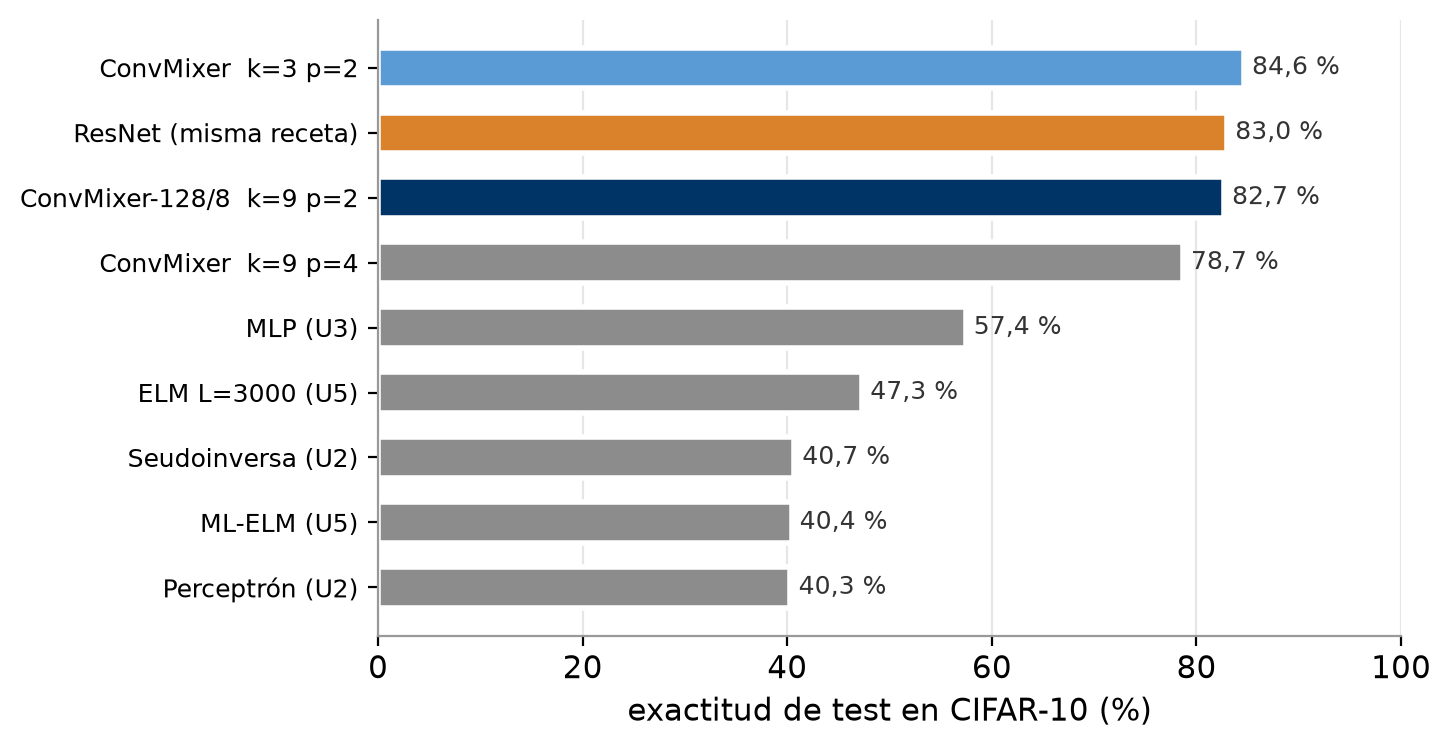
\includegraphics[width=\linewidth,height=0.70\textheight,keepaspectratio]{f_barras.png}
    \end{column}
    \begin{column}{.37\textwidth}
      \footnotesize
      \textbf{ConvMixer-128/8}: \accCMnueve\,\% con \paramsCMnueve{} parámetros.\\
      \textbf{ResNet}, misma receta: \accResNet\,\% con \paramsResNet.\\[4pt]
      El MLP tiene 16 veces más parámetros y queda 25 puntos abajo: lo que importa es el \textbf{sesgo inductivo}
      (localidad y pesos compartidos), no la cantidad de parámetros.\\[4pt]
      Lineales $\approx$ 40\,\%; la ELM mejora con más neuronas, pero sus rasgos aleatorios no ven la geometría
      de la imagen.
    \end{column}
  \end{columns}
  \fuente{\textit{Nota.} Exactitud de test (10\,000 imágenes). Modelos no convolucionales: promedio de 3 semillas. Elaboración propia.}
\end{frame}

\figslide{Curvas de validación: con 10 épocas todos siguen aprendiendo}{f_curvas_validacion.png}{\textit{Nota.} La validación se estabiliza al final porque la tasa de aprendizaje llega a cero, no porque el modelo haya terminado de aprender. Elaboración propia.}

\begin{frame}{Ablaciones frente a la Tabla 4: qué se reprodujo y qué no}
  \begin{columns}[T]
    \begin{column}{.55\textwidth}
      \centering
      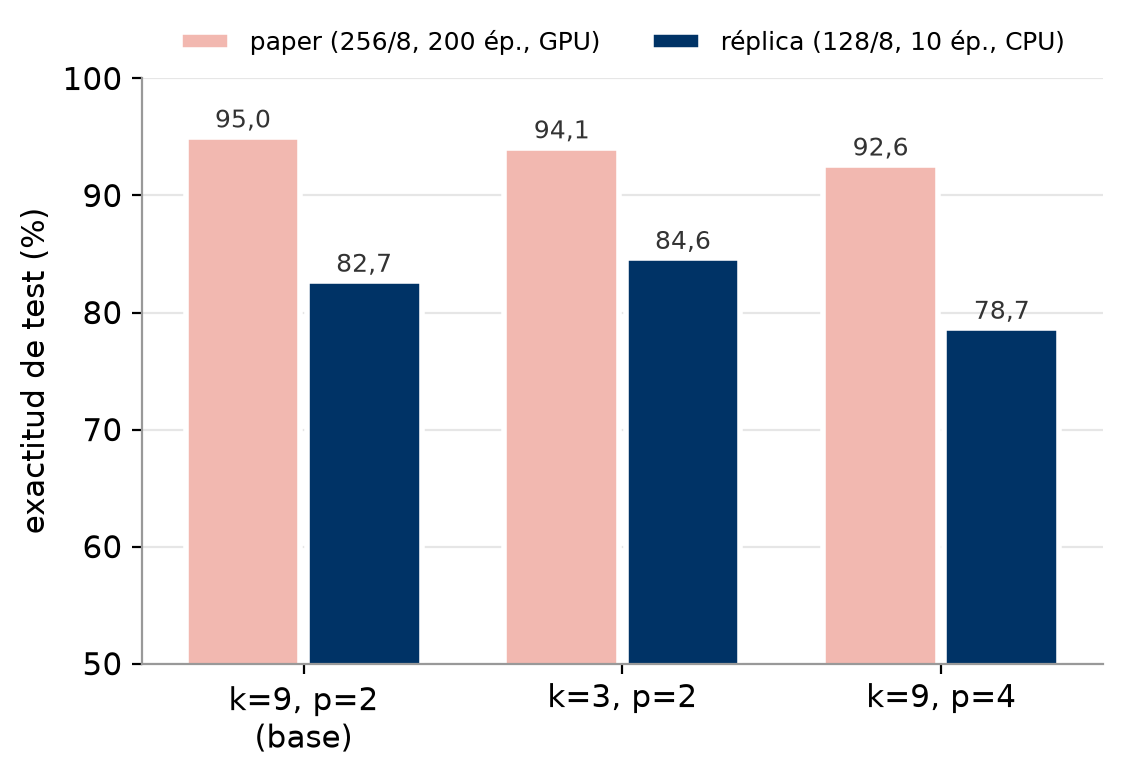
\includegraphics[width=\linewidth,height=0.66\textheight,keepaspectratio]{f_ablaciones.png}
    \end{column}
    \begin{column}{.42\textwidth}
      \footnotesize
      \textbf{Parche: se reproduce.} $p=4$ pierde \difPatch{} puntos (paper: 2,4). Menos resolución interna,
      menos detalle.\\[5pt]
      \textbf{Núcleo: no se reproduce.} $k=3$ \emph{gana} por \difKernelAbs{} puntos. Con pocas épocas converge antes
      el modelo más simple; los autores mismos dicen que el efecto de $k$ grande podría depender de entrenar más.
      Una sola semilla: indicativo, no concluyente.\\[5pt]
      \textbf{ConvMixer vs.\ ResNet}: 0,3 puntos, dentro del ruido. La ventaja del paper aparece en ImageNet con
      modelos 100 veces más grandes.
    \end{column}
  \end{columns}
  \fuente{\textit{Nota.} Réplica: ConvMixer-128/8, 10 épocas, CPU. Artículo: ConvMixer-256/8, 200 épocas, GPU (Trockman y Kolter, 2023, Tabla 4).}
\end{frame}

\begin{frame}{El costo sí se reproduce: el ConvMixer es lento}
  \begin{columns}[T]
    \begin{column}{.56\textwidth}
      \centering
      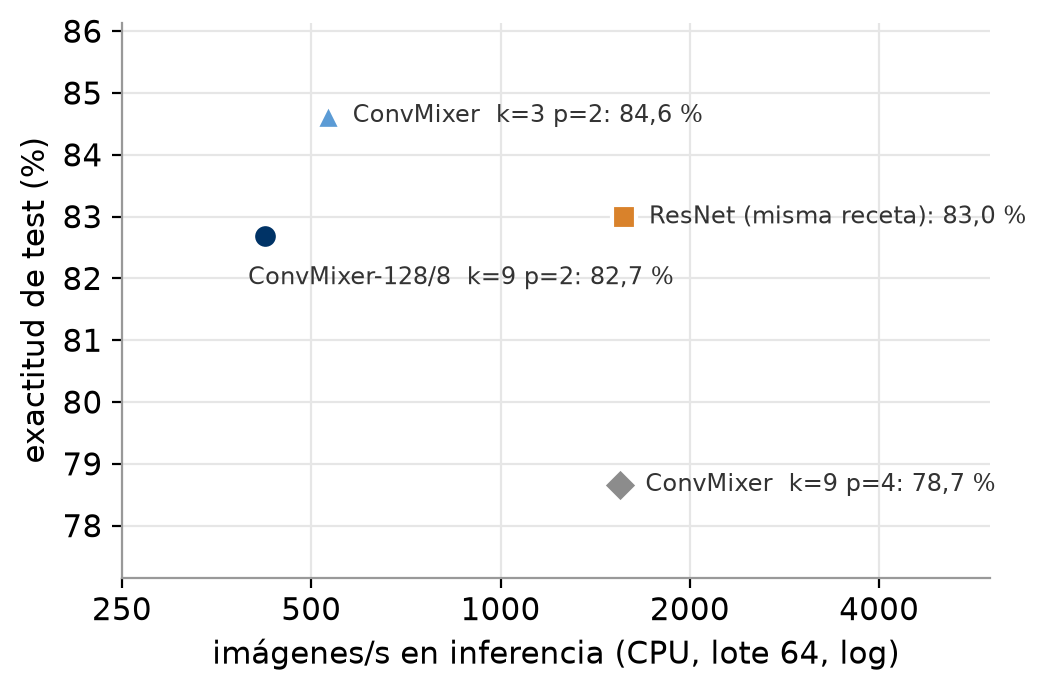
\includegraphics[width=\linewidth,height=0.68\textheight,keepaspectratio]{f_throughput.png}
    \end{column}
    \begin{column}{.40\textwidth}
      \bignum{\ratioTput$\times$}{más rápida la ResNet en inferencia\\(\tputResNet{} frente a \tputCMnueve{} imágenes/s en CPU)}
      \vspace{8pt}
      {\footnotesize Entrenamiento: 110 min el ConvMixer, 32 min la ResNet. La convolución depthwise de núcleo
      grande sobre una resolución interna alta está poco optimizada, igual que lo admiten los autores (Tablas 1 y 2).}
    \end{column}
  \end{columns}
  \fuente{\textit{Nota.} Lote de 64 imágenes, misma CPU de 8 núcleos, eje logarítmico. Elaboración propia.}
\end{frame}

\begin{frame}{¿Y si le doy el cómputo del paper? Réplica en GPU (Google Colab)}
  \begin{columns}[T]
    \begin{column}{.58\textwidth}
      \centering
      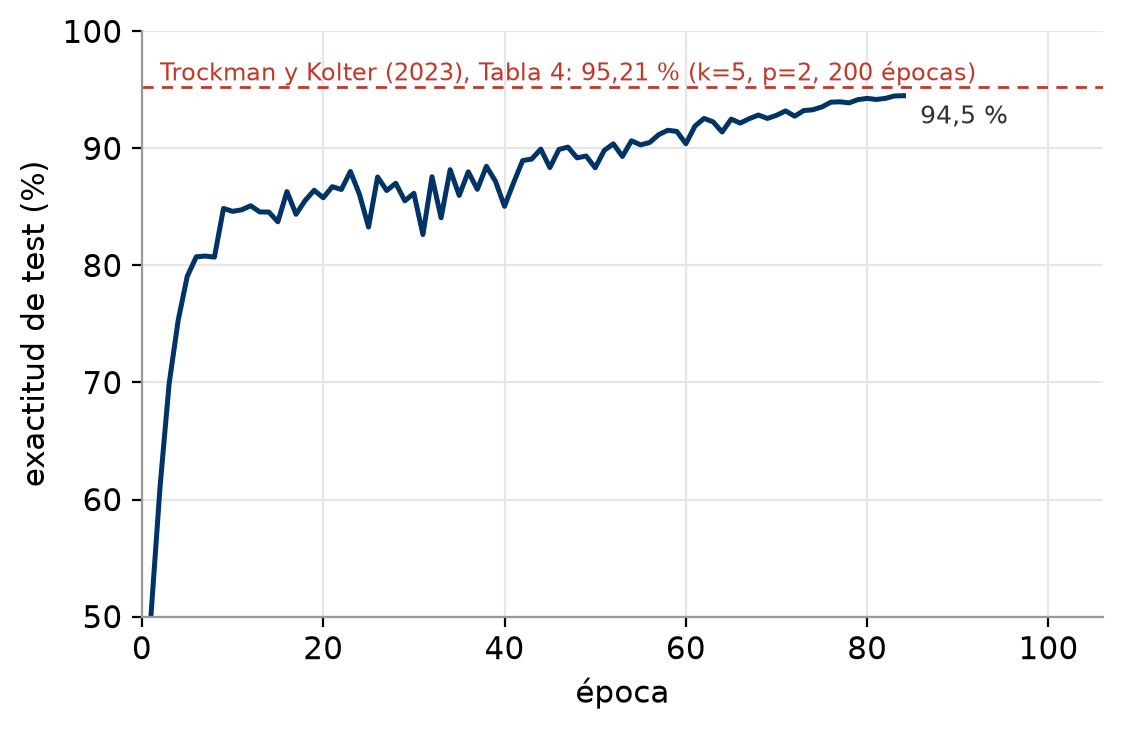
\includegraphics[width=\linewidth,height=0.66\textheight,keepaspectratio]{f_colab.png}
    \end{column}
    \begin{column}{.39\textwidth}
      \bignum{\accColab\,\%}{ConvMixer-256/8, $k=5$, $p=2$, receta oficial de los autores\\(paper: 95,21\,\%)}
      \vspace{6pt}
      {\footnotesize GPU T4 gratuita, unos \segColab{} s por época con RandAugment, ColorJitter y \emph{random
      erasing}. La brecha de la réplica en CPU se explica por la escala, no por la implementación.}
    \end{column}
  \end{columns}
  \fuente{\textit{Nota.} Receta de \texttt{github.com/locuslab/convmixer-cifar10} (Trockman y Kolter, 2023). Se informa la última época, \colabNota.}
\end{frame}

\begin{frame}{CPU frente a GPU: el cómputo y la receta pesan más que la arquitectura}
  \centering\footnotesize
  \resizebox{\linewidth}{!}{\begin{tabular}{lcccc}
    \toprule
     & \textbf{CPU propia} & \textbf{Colab (T4)} & \textbf{Kaggle (T4)} & \textbf{Artículo (GPU)}\\
    \midrule
    Modelo & 128/8, $k$=9, $p$=2 & 256/8, $k$=5, $p$=2 & 256/8, $k$=5, $p$=2 & 256/8, $p$=2\\
    Parámetros & 223\,k & 594\,k & 594\,k & 709\,k / 594\,k\\
    Receta & escalado, recorte, espejo & + RandAugment, borrado & + mixup, CutMix, wd 0 & \texttt{timm} + mixup, CutMix\\
    Épocas & \epocasCNN & \epColab & \epKaggle & 200\\
    Tiempo por época & \minEpCPU{} min & \segColab{} s & \segKaggle{} s & --\\
    Tiempo total & \minCMnueve{} min & \minColab{} min & \minKaggle{} min & --\\
    \rowcolor{unajgris}\textbf{Exactitud de test} & \textbf{\accCMnueve\,\%} & \textbf{\accColab\,\%} & \textbf{\accKaggle\,\%} & \textbf{95,0 / 95,21\,\%}\\
    \bottomrule
  \end{tabular}}
  \vspace{6pt}
  \begin{columns}[T]
    \begin{column}{.48\textwidth}\footnotesize
      \textbf{Lectura}: con la receta del artículo (200 épocas, mixup, CutMix) la réplica \textbf{iguala} el valor
      publicado: \accKaggle\,\% frente a 95,21\,\%. Con una sola semilla, los 0,27 puntos de diferencia no
      son una mejora demostrada.
    \end{column}
    \begin{column}{.48\textwidth}\footnotesize
      \textbf{Para el debate}: Kaggle fue más del doble de rápido por época con la misma GPU (no sé a qué se debe).
      Colab nos negó la GPU por límite de uso y cortó una corrida en la época 84. ¿Cuánto de ``el mejor modelo'' es
      ``el que más cómputo recibió''?
    \end{column}
  \end{columns}
  \fuente{\textit{Nota.} Una corrida por configuración. Se informa la última época. Valores del artículo: Trockman y Kolter (2023, Tabla 4). Elaboración propia.}
\end{frame}



% =================================================================
\section{Reflexión}
\begin{frame}{Reflexión crítica}
  \begin{columns}[T]
    \begin{column}{.48\textwidth}
      \small
      \textbf{¿Por qué este artículo?} Es bibliografía que trabajé en el ITBA; tiene una pregunta científica
      clara y es replicable en hardware modesto; y se conecta con mi tesis (IA para la evaluación de la
      inestabilidad espinal), donde elegir entre CNN y transformers con pocos datos es una decisión real.\\[4pt]
      \textbf{Otros dominios}: segmentación médica (la resolución interna alta conserva detalle anatómico),
      microscopía, teledetección, señales 1D (ECG) y espectrogramas.\\[4pt]
      \textbf{Conocimientos previos}: U3 (retropropagación, optimización), U4 (convolución, SGD), U1 (validación);
      depthwise, BatchNorm, residuales, AdamW, aumentación, atención y ViT.
    \end{column}
    \begin{column}{.48\textwidth}
      \begin{alertblock}{Ética}
        \footnotesize
        \begin{itemize}
          \item \textbf{Cómputo}: unos 90 días-GPU por un punto de ImageNet; sin GPU sólo se verifica una versión
          reducida, y la investigación se concentra en quien tiene hardware.
          \item \textbf{Reproducibilidad}: el código abierto ayuda; una sola corrida y el ajuste sobre el test, no.
          \item \textbf{Sesgos}: ImageNet no representa a todas las poblaciones; en medicina hace falta validación
          externa local.
          \item \textbf{Doble uso}: la misma tecnología sirve para diagnóstico y para vigilancia.
        \end{itemize}
      \end{alertblock}
    \end{column}
  \end{columns}
\end{frame}

\begin{frame}{Conclusiones}
  \begin{columns}[T]
    \begin{column}{.48\textwidth}
      \begin{block}{Sobre el artículo}
        \footnotesize
        \begin{itemize}
          \item La idea es fuerte y simple: una CNN con parches y diseño isotrópico compite con los transformers.
          \item La evidencia es parcial: sin diseño factorial, con recetas distintas entre modelos y una sola corrida
          por configuración.
          \item Sí muestra algo valioso: la receta de entrenamiento pesa tanto como la arquitectura.
        \end{itemize}
      \end{block}
    \end{column}
    \begin{column}{.48\textwidth}
      \begin{block}{Sobre la réplica}
        \footnotesize
        \begin{itemize}
          \item Con la receta oficial en GPU: \accColab\,\% (paper: 95,21\,\%). La implementación es correcta.
          \item Con poco cómputo: ConvMixer $\approx$ ResNet (\accCMnueve{} vs.\ \accResNet\,\%), pero la ResNet es
          \ratioTput{} veces más rápida.
          \item Se reproduce el efecto del parche; el del núcleo grande, no con 10 épocas.
          \item Modelos del curso: lineal $\approx$ 40 $<$ ELM 47 $<$ MLP 57 $\ll$ CNN 83--85\,\%.
        \end{itemize}
      \end{block}
    \end{column}
  \end{columns}
  \clave{Replicar no es copiar un número: es seguir el procedimiento, medir lo mismo y poder explicar cada
  diferencia. Aquí cada brecha tiene una causa concreta: épocas, tamaño, aumentación o la semilla.}
\end{frame}


\begin{frame}{Reproducibilidad y referencias}
  \begin{columns}[T]
    \begin{column}{.5\textwidth}\footnotesize
      \textbf{Repositorio}: \texttt{src/} (modelos, entrenamiento, experimentos, figuras), \texttt{config.json}
      (todas las semillas e hiperparámetros), \texttt{results/} (JSON y pesos),
      \texttt{notebooks/replica\_convmixer.ipynb} (corre en Colab con GPU, o en modo rápido en CPU).\\[4pt]
      Todo número de estas diapositivas se genera desde \texttt{results/*.json}.\\[4pt]
      \textbf{Asistente de IA}: el código y el texto se prepararon con Claude Code. La verificación fue mía: la
      ec.~(4) contra el conteo de PyTorch y el test evaluado una sola vez.
    \end{column}
    \begin{column}{.46\textwidth}\fontsize{5}{6}\selectfont
      \textbf{Referencias (APA 7)}\par\vspace{2pt}
      \hangindent=1em Dosovitskiy, A. et al.\ (2021). An image is worth 16x16 words: Transformers for image recognition at scale. \emph{ICLR}. https://doi.org/10.48550/arXiv.2010.11929\par
      \hangindent=1em Freund, Y. y Schapire, R. E. (1999). Large margin classification using the perceptron algorithm. \emph{Machine Learning, 37}(3), 277--296.\par
      \hangindent=1em He, K., Zhang, X., Ren, S. y Sun, J. (2016). Deep residual learning for image recognition. \emph{CVPR}, 770--778. https://doi.org/10.1109/CVPR.2016.90\par
      \hangindent=1em Huang, G.-B., Zhu, Q.-Y. y Siew, C.-K. (2006). Extreme learning machine: Theory and applications. \emph{Neurocomputing, 70}(1--3), 489--501. https://doi.org/10.1016/j.neucom.2005.12.126\par
      \hangindent=1em Kasun, L. L. C., Zhou, H., Huang, G.-B. y Vong, C. M. (2013). Representational learning with ELMs for big data. \emph{IEEE Intelligent Systems, 28}(6), 31--34.\par
      \hangindent=1em Krizhevsky, A. (2009). \emph{Learning multiple layers of features from tiny images} [Informe técnico]. University of Toronto. https://www.cs.toronto.edu/\textasciitilde kriz/cifar-10.html\par
      \hangindent=1em Liu, Z. et al.\ (2021). Swin Transformer. \emph{ICCV}, 10012--10022. https://doi.org/10.48550/arXiv.2103.14030\par
      \hangindent=1em Sandler, M., Baccash, J., Zhmoginov, A. y Howard, A. (2019). Non-discriminative data or weak model? \emph{ICCV Workshops}.\par
      \hangindent=1em Tolstikhin, I. et al.\ (2021). MLP-Mixer: An all-MLP architecture for vision. \emph{NeurIPS, 34}, 24261--24272.\par
      \hangindent=1em Touvron, H. et al.\ (2021). Training data-efficient image transformers \& distillation through attention. \emph{ICML}, 10347--10357.\par
      \hangindent=1em Trockman, A. y Kolter, J. Z. (2023). Patches are all you need? \emph{Transactions on Machine Learning Research}. https://doi.org/10.48550/arXiv.2201.09792\par
    \end{column}
  \end{columns}
\end{frame}

\begin{frame}[plain]
  \centering\vfill
  {\Large\bfseries\color{unajazul}¡Gracias!}\\[8pt]
  {\small Preguntas y debate}\\[14pt]
  
\includegraphics[height=1.3cm]{logo_unaj.png}
  \vfill
\end{frame}

% =================================================================
\appendix
% Anexo (para preguntas)
\begin{frame}[fragile]{Anexo A: el modelo completo en PyTorch (Fig.~7 del artículo)}
\begin{columns}[T]
\begin{column}{.56\textwidth}
\scriptsize
\begin{verbatim}
def ConvMixer(dim, depth, kernel_size=9,
              patch_size=7, n_classes=1000):
  return nn.Sequential(
    nn.Conv2d(3, dim, kernel_size=patch_size,
              stride=patch_size),
    nn.GELU(), nn.BatchNorm2d(dim),
    *[nn.Sequential(
        Residual(nn.Sequential(
          nn.Conv2d(dim, dim, kernel_size,
                    groups=dim, padding="same"),
          nn.GELU(), nn.BatchNorm2d(dim))),
        nn.Conv2d(dim, dim, kernel_size=1),
        nn.GELU(), nn.BatchNorm2d(dim)
      ) for i in range(depth)],
    nn.AdaptiveAvgPool2d((1,1)), nn.Flatten(),
    nn.Linear(dim, n_classes))
\end{verbatim}
\end{column}
\begin{column}{.40\textwidth}
\small
\textbf{Verificación de la ec.~(4)} (PyTorch = fórmula):\\[3pt]
\begin{tabular}{lr}
\toprule
Modelo & Parámetros\\
\midrule
256/8, $k$=9, $p$=1 & 706\,570\\
256/8, $k$=9, $p$=2 & 708\,874\\
128/8, $k$=9, $p$=2 & 223\,370\\
128/8, $k$=3, $p$=2 & 149\,642\\
\bottomrule
\end{tabular}\\[4pt]
{\footnotesize Coinciden con la Tabla~4 del artículo (707\,k y 709\,k).}
\end{column}
\end{columns}
\end{frame}

\begin{frame}{Anexo B: los modelos de las otras unidades, en una línea cada uno}
\small
\begin{tabularx}{\textwidth}{lX}
\toprule
\textbf{U2 Seudoinversa} & $W=V\,\mathrm{diag}\!\big(\tfrac{\sigma_i}{\sigma_i^2+\lambda}\big)U^\top T$ sobre
3\,072 píxeles + sesgo; $\lambda$ por validación cruzada de 5 pliegues, con una SVD por pliegue.\\
\textbf{U2 Perceptrón} & Una neurona escalón por clase; si se equivoca, $w_{y}\mathrel{+}=x$ y $w_{\hat y}\mathrel{-}=x$;
pesos promediados (Freund y Schapire, 1999).\\
\textbf{U3 MLP} & 3072--1024--512--10, ReLU, \emph{dropout} 0,2, AdamW + programa triangular, 15 épocas.\\
\textbf{U5 ELM} & $H=\mathrm{ReLU}(XA+b)$ con $A,b$ aleatorios fijos; $\beta=H^+T$ (Tikhonov); $L\in\{500,\dots,3000\}$.\\
\textbf{U5 ML-ELM} & Dos ELM-autoencoders (1\,000 + 1\,000, pesos ortogonales) + ELM de 3\,000 (Kasun et al., 2013).\\
\textbf{U4 ResNet} & Tallo $3\times3$ + 3 bloques residuales (32, 64, 128 canales; resolución $32\to16\to8$),
\emph{pooling} global; misma receta que el ConvMixer.\\
\bottomrule
\end{tabularx}
\end{frame}

\figslide{Anexo C: curva de validación cruzada de la seudoinversa (U1 + U2)}{f_cv_lineal.png}{\textit{Nota.} Exactitud media $\pm$ desvío en 5 pliegues de las 45\,000 imágenes de entrenamiento. El test se usa una sola vez, con el $\lambda$ elegido.}

\figslide{Anexo D: matriz de confusión del ConvMixer-128/8 (test, \% por fila)}{f_confusion.png}{\textit{Nota.} Las confusiones se concentran entre clases parecidas: perro con gato (13\,\%) y gato con perro (12\,\%); los animales chicos se confunden con rana y el camión con el auto. Gato es la clase más difícil (62\,\% de acierto). Elaboración propia.}

\figslide{Anexo E: filtros del embebido de parches (cf.\ Apéndice C del artículo)}{f_filtros.png}{\textit{Nota.} 64 filtros RGB de $4\times4$ del ConvMixer con $p=4$: bordes orientados y manchas de color, como los que describen Trockman y Kolter (2023). Elaboración propia.}


\end{document}
